\section{1184071 - Annisa Khairani Febrianti}
\subsection{Teori}
\begin{enumerate}

	\item Jelaskan apa itu Binary Classification dilengkapi dengan ilustrasi gambar sendiri.
	\hfill\break
Binary Classification merupakan sebuah tugas yang mengklafisikan himpunan didalamnya dan terdapat elemen-elemen yang dimasukkan ke dalam kelompok berdasarkan aturan klasifikasi. Adapun katakteristik contohnya pada tes medis digunakan untuk mengetahui suatu pasien memiliki penyakit tertentu atau tidak. dan properti klasifikasi tersebut adalah keberadaan penyakit dari pasien.\\
Binary Classification digunakan untuk tujuan praktis dalam banyak masalah klasifikasi biner, dan kedua kelompok tersebut tidak simetris daripada akurasi secara keseluruhan, proporsi relatif dari berbagai macam kesalahan yang menarik. Contohnya, dalam pengujian medis tadi, false positif maksudnya mendeteksi penyakit ketika ada sedangkan untuk false negatif artinya tidak mendeteksi penyakit ketika ada.\\
Ada banyak metrik yang bisa digunakan dalam mengukur kinerja klasifikasi dan prediksi. Contohnya seperti gambar dibawah ini :

	\begin{figure}[h]
	\centering
		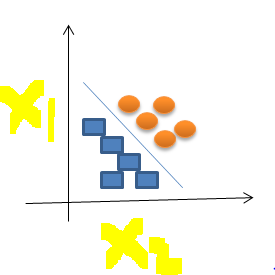
\includegraphics[width=4cm]{figures/1184071/chapter2/1.PNG}
		\caption{Binary classification.}
	\end{figure}

	\item Jelaskan apa itu supervised learning dan unsupervised learning dan clustering dengan ilustrasi gambar sendiri.
	\hfill\break

	\begin{itemize}
		\item Supervised Learning
		\hfill\break Dalam Supervised Learning, suatu program komputer diberikan dataset pelatihan yang kemudian diberi label dengan nilai output yang sesuai, dan fungsi tersebut akan ditentukan berdasarkan pada dataset. Fungsi algoritma tersebut kemudian akan digunakan untuk mengklasifikasian data baru untuk memprediksi nilai-nilai output yang sesuai dengan asumsi bahwa data baru sesuai dengan aturan dan fungsi yang digunakan. Contohnya seperti gambar dibawah ini :
		
		\begin{figure}[h]
		\centering
			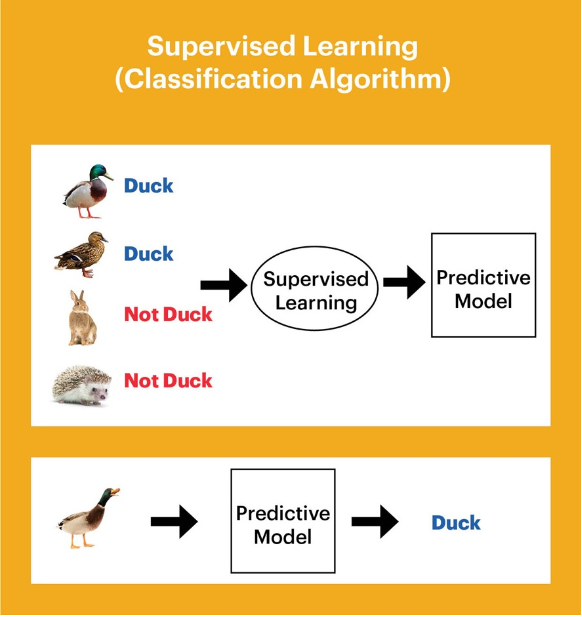
\includegraphics[width=8cm]{figures/1184071/chapter2/2.PNG}
			\caption{Supervised Learning.}
		\end{figure}

		\newpage\item Unsupervised Learning 
		\hfill\break
		Berbeda dengan Supervised Learning, Unsupervised Learning  merupakan algoritma yang tidak memiliki attribut tambahan yang akan diprediksi melainkan dengan melihat kesamaan dari atrribut-atribut yang dimiliki. Contohnya seperti gambar dibawah ini :

		\begin{figure}[h]
		\centering
			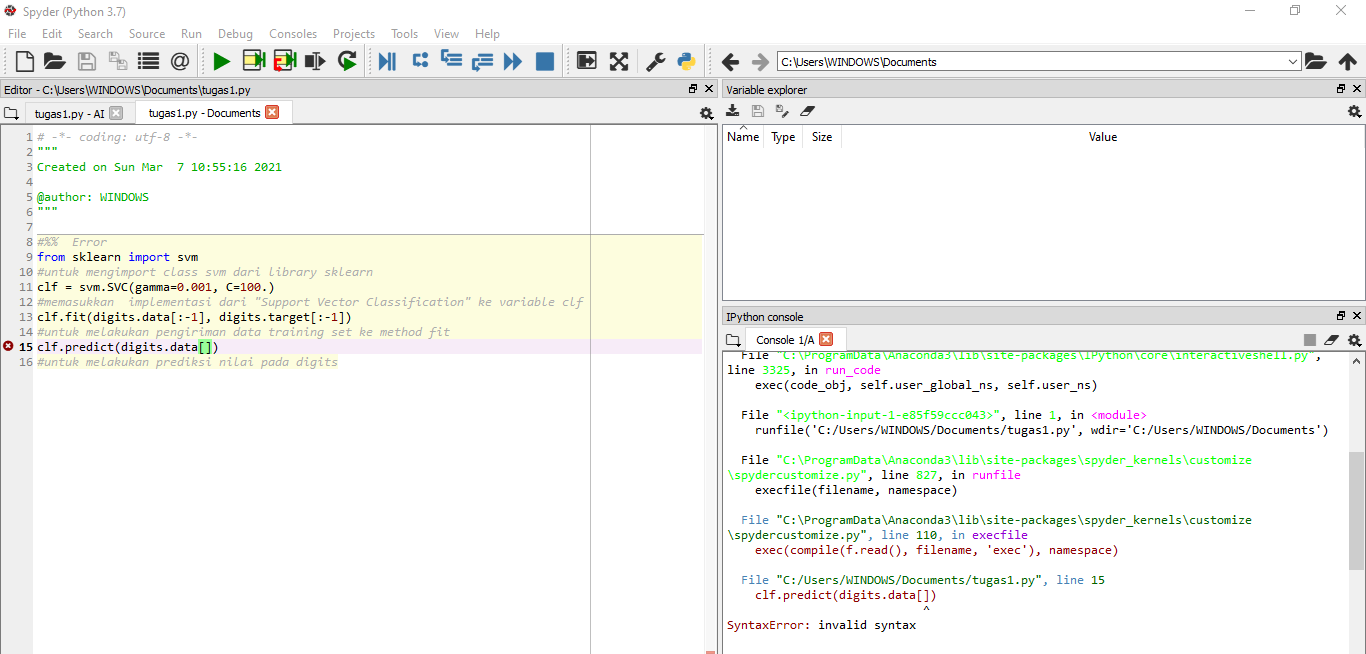
\includegraphics[width=8cm]{figures/1184071/chapter2/3.PNG}
			\caption{Unsupervised Learning.}
		\end{figure}

		\item Clustering
		\hfill\break
		Clustering merupakan suatu teknik yang masuk kedalam kelompok Unsupervised Learning yang  merupakan teknik dimana mesin akan bekerja atau belajar sendiri tanpa diajari bagaimana cara memecahkan suatu masalah. Contohnya, Kita memiliki sebuah data, yaitu data pelanggan yang berisi jenis kelamin, besarnya penghasilan dan besarnya pembelian produk. Maka dengan algoritma Clustering kita dapat mengetahui pelanggan kita akan dikelompokkan kedalam beberapa kluster dengan sendirinya.Misalnya ada pelanggan yang pelit,pelanggan yang royal dan lain sebagainya. Contohnya, Bisa kita lihat bagaimana sebuah teknik clustering bisa mengelompokkan data ke dalam beberapa kluster. Contohnya seperti gambar dibawah ini :
		\begin{figure}[h]
		\centering
			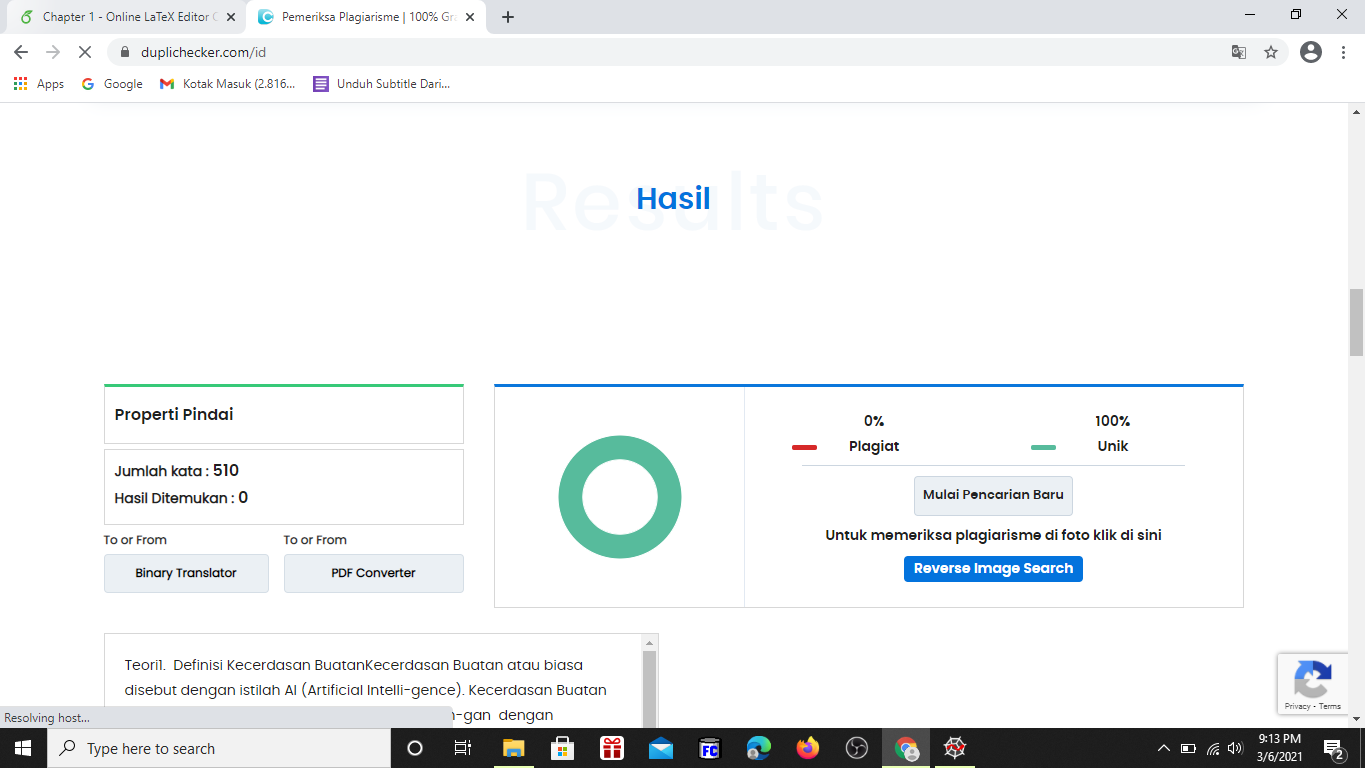
\includegraphics[width=8cm]{figures/1184071/chapter2/4.PNG}
			\caption{Clustering.}
		\end{figure}
	\end{itemize}
	
	\item Jelaskan apa itu evaluasi dan akurasi dari buku dan disertai ilustrasi contoh dengan gambar sendiri.
	\hfill\break
	Evaluasi merupakan suatu cara atau teknik dalam mengevaluasi seberapa baik model bekerja dengan mengukur akurasinya. Sedangkan akurasi adalah suatu persentase kasus yang diklasifikasikan dengan benar. Kita bisa menganalisis suatu kesalahan yang dibuat dengan model atau tingkat confusion dengan menggunakan matriks confusion. Berikut adalah contoh klasifikasi biner yang menunjukkan berapa kali model telah membuat prediksi yang benar dari objek.
	\begin{figure}[h]
	\centering
		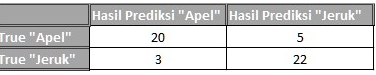
\includegraphics[width=10cm]{figures/1184071/chapter2/5.PNG}
		\caption{Evaluasi dan Akurasi.}
	\end{figure}

	\item Jelaskan bagaimana cara membuat dan membaca confusion matrix, buat confusion matrix buatan sendiri.
	\\ \textbf{Confusion Matrix} adalah suatu matrix yang memberikan informasi perbandingan hasil klasifikasi yang dilakukan pada sistem atau model dengan hasil klasifikasi sebenarnya. Confusion Matrix berbentuk tabel matriks yang menggambarkan suatu kinerja model klasifikasi dari serangkaian data uji yang nilai sebenarnya diketahui.
	\hfill\break
	\begin{enumerate}
	\item Cara membuat dan membaca confusion matrix :
	\begin{itemize}
	\item Tentukan pokok permasalahan dan atributanya, misal gaji dan listrik.
	\item Buat pohon keputusan
	\item Lalu data testingnya
	\item Lalu mencari nilai a, b, c, dan d. Semisal a = 5, b = 1, c = 1, dan d = 3.
	\item Selanjutnya mencari nilai recall, precision, accuracy, serta dan error rate.
	\end{itemize}
	\item Berikut adalah contoh dari confusion matrix :
	\begin{itemize}
	\item Recall =3/(3+3) = 0,5
	\item Precision = 3/(3+5) = 0,375
	\item Accuracy =(3+5)/(3+5+5+3) = 0,5
	\end{itemize}
	\end{enumerate}

	\begin{figure}[h]
	\centering
		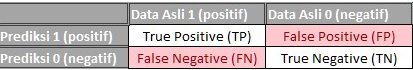
\includegraphics[width=8cm]{figures/1184071/chapter2/6.PNG}
		\caption{Confusion Matrix.}
	\end{figure}

	\item Jelaskan bagaimana K-fold cross validation bekerja dengan gambar ilustrasi contoh buatan sendiri.
	\hfill\break
	\begin{itemize}
	\item Total instance dibagi menjadi N bagian.
	\item Fold yang pertama adalah bagian pertama menjadi data uji (testing data) dan sisanya menjadi training data.
	\item Lalu hitung akurasi berdasarkan porsi data tersebut dengan menggunakan persamaan.
	\item Fold yang ke dua adalah bagian ke dua menjadi data uji (testing data) dan sisanya training data. 
	\item Kemudian hitung akurasi berdasarkan porsi data tersebut.
	\item Dan seterusnya hingga habis mencapai fold ke-K.
	\item Terakhir hitung rata-rata akurasi K buah.
	\end{itemize}

	\begin{figure}[h]
	\centering
		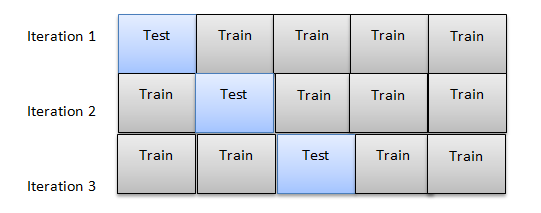
\includegraphics[width=7cm]{figures/1184071/chapter2/7.PNG}
		\caption{K-fold Cross Validation.}
	\end{figure}

	\item Jelaskan apa itu decision tree dengan gambar ilustrasi contoh buatan sendiri.
	\hfill\break
	Decision Tree merupakan suatu model yang diprediksi dengan menggunakan struktur pohon atau strktur yang berhirarki. Konsepnya adalah mengubah data menjadi decesion tree dan beberapa aturan keputusan. Decicion Tree memiliki manfaat yaitu membrekdown porses pengambilan keputusan yang kompleks menjadi lebih simpel sehingga pengambil keputusan akan lebih mengintrpretasikan solusi dari suatu permasalahan.

	\begin{figure}[h]
	\centering
		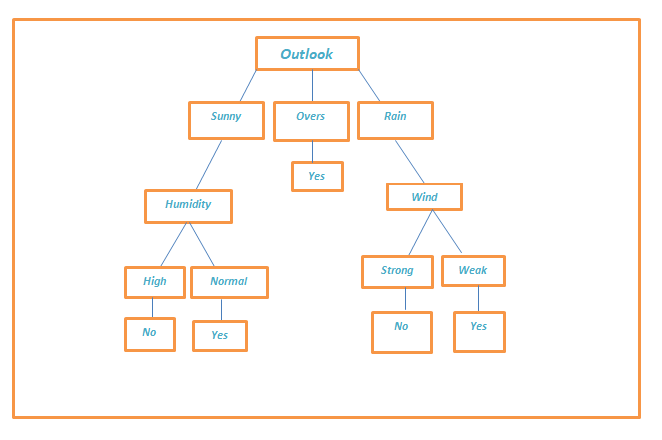
\includegraphics[width=9cm]{figures/1184071/chapter2/8.PNG}
		\caption{Decision Tree.}
	\end{figure}

	\item Jelaskan apa itu information gain dan entropi dengan gambar ilustrasi buatan sendiri.
	\hfill\break
		Information Gain merupakan suatu teknik yang didasarkan pada penurunan entropi setelah dataset dibagi pada atribut untuk membangun keputusan dan menemukan atribut yang mengembalikan perolehan informasi tertinggi. Sedangkan Entropi adalah suatu ukuran acak dalam informasi yang sedang diproses.Semakin tinggi entropi, semakin sulit untuk menarik kesimpulan dari informasi itu. Membalik koin adalah contoh tindakan yang memberikan informasi acak. Untuk koin yang tidak memiliki afinitas terhadap kepala atau ekor, hasil lemparannya sulit diprediksi. Mengapa Karena tidak ada hubungan antara yang menentang dan hasil. Dari penjelasan diatas inilah inti dari entropi.
	\begin{figure}[h]
	\centering
		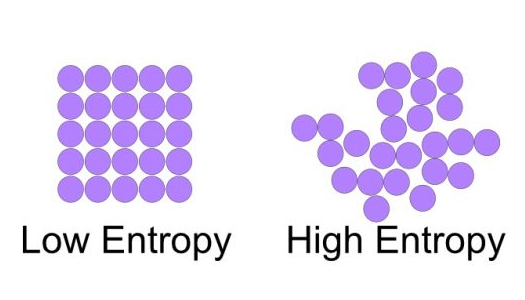
\includegraphics[width=10cm]{figures/1184071/chapter2/9.PNG}
		\caption{Entropi.}
	\end{figure}
\end{enumerate}

\subsection{Praktek}
\begin{enumerate}
	\item Soal 1
	\hfill\break
	\lstinputlisting[firstline=8, lastline=20]{src/1184071/chapter2/1184071.py}
	Kode di atas digunakan untuk mengimpor atau mengirim library pandas sebagai pd. Kemudian ditentukan variabel "Jambi" untuk dipanggil dataset diperoleh dari data student-mat.csv. Hasilnya adalah sebagai berikut :
	\begin{figure}[h]
	\centering
		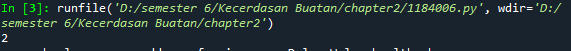
\includegraphics[width=10cm]{figures/1184071/chapter2/1-m.PNG}
		\caption{Hasil Soal 1.}
	\end{figure}
	\item Soal 2
	\hfill\break
	\lstinputlisting[firstline=21, lastline=33]{src/1184071/chapter2/1184071.py}
	Kode di atas ada bagian mendeklarasikan pass/fail nya data berdasarkan G1+G2+G3. Dengan ketentuan nilai pass nya yaitu sama dengan 30. kemudian pada variabel medan dideklarasikan jika baris dengan G1+G2+G3 ditambahkan, dan hasilnya sama dengan 35 maka axisnya 1. Hasilnya adalah sebagai berikut :
	\begin{figure}[h]
	\centering
		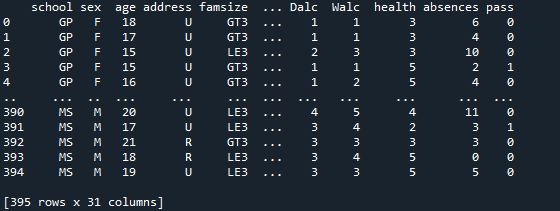
\includegraphics[width=8cm]{figures/1184071/chapter2/2-m.PNG}
		\caption{Hasil Soal 2.}
	\end{figure}
	\item Soal 3
	\hfill\break
	\lstinputlisting[firstline=34, lastline=41]{src/1184071/chapter2/1184071.py}
	One-hot encoding merupakan suatu proses yang dimana variabel kategorikal dikonversi menjadi bentuk yang dapat disediakan untuk algoritma ML untuk melakukan pekerjaan yang lebih baik dalam prediksi. Metode head ini digunakan untuk mengembalikan baris n atas 5 secara default dari frame atau seri data Karena saya memuat data menggunakan. Hasilnya adalah sebagai berikut :
	\begin{figure}[h]
	\centering
		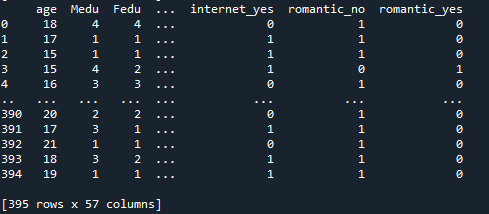
\includegraphics[width=8cm]{figures/1184071/chapter2/3-m.PNG}
		\caption{Hasil Soal 3.}
	\end{figure}
	\item Soal 4
	\hfill\break
	\lstinputlisting[firstline=42, lastline=70]{src/1184071/chapter2/1184071.py}
	Sample digunakan untuk mengembalikan sampel acak item dari suatu objek. Pada bagian tersebut, terdapat train dan test yaing digunakan untuk untuk membagi train, test dan kemudian membagi lagi train ke validasi dan test. Kemudia akan mengimport module numpy sebagai np yang akan digunakan untuk mengembalikan nilai passing dari pelajar dari keseluruhan dataset dengan cara print. Hasilnya adalah sebagai berikut :
	\begin{figure}[h]
	\centering
		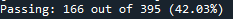
\includegraphics[width=8cm]{figures/1184071/chapter2/4-m.PNG}
		\caption{Hasil Soal 4.}
	\end{figure}
	\item Soal 5
	\hfill\break
	\lstinputlisting[firstline=72, lastline=81]{src/1184071/chapter2/1184071.py}
	Dari librari scikitlearn import modul tree. Kemudian definisikan variabel asahan dengan menggunakan DecisionClassifier. Kemudian pada variabel asahan terdapat Criterion yaitu suatu fungsi untuk mengukur kualitas split, setelah itu agar DecisionTreeClassifier dapat dijalankan gunakan perintah fit. Hasilnya adalah sebagai berikut :
	\begin{figure}[h]
	\centering
		
\includegraphics[width=10cm]{figures/1184071/chapter2/5-m.PNG}
		\caption{Hasil Soal 5.}
	\end{figure}
\item Soal 6
	\hfill\break
	\lstinputlisting[firstline=82, lastline=92]{src/1184071/chapter2/1184071.py}
	\textit{Graphviz} merupakan sebuah perangkat lunak yang memvisualisasi grafik open source. Visualisasi grafik juga memiliki arti yaitu cara mewakili informasi struktural sebagai diagram grafik dan jaringan abstrak. Hasilnya adalah sebagai berikut :
	\begin{figure}[h]
	\centering
		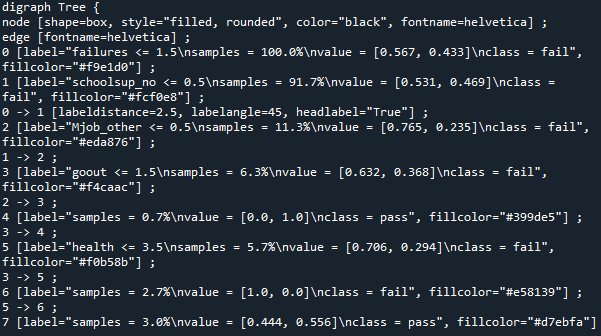
\includegraphics[width=10cm]{figures/1184071/chapter2/6-m.PNG}
		\caption{Hasil Soal 6.}
	\end{figure}
	\item Soal 7
	\hfill\break
	\lstinputlisting[firstline=93, lastline=96]{src/1184071/chapter2/1184071.py}
	\textit{Tree.export graphviz} merupakan fungsi yang menghasilkan suatu representasi Graphviz dari decision tree, yang kemudian ditulis ke dalam outfile setelah selesai akan menyimpan classifilenya dan diekspor kedalam file student performance, apabila terjadi kesalahan akan mengembalikan nilai failed. 

	\item Soal 8
	\hfill\break
	\lstinputlisting[firstline=98, lastline=100]{src/1184071/chapter2/1184071.py}
	Score disebut dengan prediksi yang merupakan sebuah proses yang menghasilkan nilai berdasarkan model pembelajaran mesin yang terlatih, diberi beberapa data input baru. Nilai atau skor yang dibuat dapat mewakili prediksi nilai masa depan, tetapi mereka juga mungkin mewakili kategori atau hasil yang mungkin. Jadi disini asahan akan memprediksi nilai dari medan test att dan test pass .
    \item Soal 9
	\hfill\break
	\lstinputlisting[firstline=101, lastline=109]{src/1184071/chapter2/1184071.py}
	Skrip ini akan mengevaluasi score dengan memvalidasi silang. Dimana variabel scores tersebut berisikan crossvalscore yang berfungi untuk pembantu pada estimator dan dataset. Kemudian akan menampilkan score rata-rata dan kurang lebih dua standar deviasi yang mencakup 95 persen score. 
	\item Soal 10
	\hfill\break
	\lstinputlisting[firstline=111, lastline=119]{src/1184071/chapter2/1184071.py}
	Pada skrip ini menunjukkan seberapa dalam tree itu. Semakin dalam tree, semakin banyak perpecahan yang dimilikinya dan menangkap lebih banyak informasi tentang data. variabel asahan akan mendefinisikan tree nya yang kemudian variabel scores akan mengevaluasi score dengan validasi silang. disini mendefinisikan decision tree dengan kedalaman mulai dari 1 hingga 20. Hasilnya adalah sebagai berikut :
	\begin{figure}[h]
	\centering
		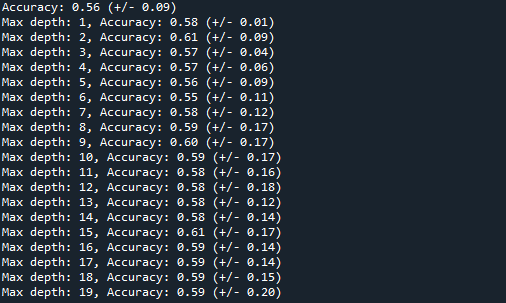
\includegraphics[width=10cm]{figures/1184071/chapter2/10-m.PNG}
		\caption{Hasil Soal 10.}
	\end{figure}
\item Soal 11
	\hfill\break
	\lstinputlisting[firstline=121, lastline=144]{src/1184071/chapter2/1184071.py}
	Depth acc akan membuat array kosong dengan mengembalikan array baru dengan bentuk dan tipe yang diberikan, tanpa menginisialisasi entri. Dengan 19 sebagai bentuk array kosong, 3 sebagai output data-type dan float urutan kolomutama (gaya Fortran) dalam memori. variabel asahan yang akan melakukan split score akan mengvalidasi score secara silang. Hasilnya adalah sebagai berikut :
	\begin{figure}[h]
	\centering
		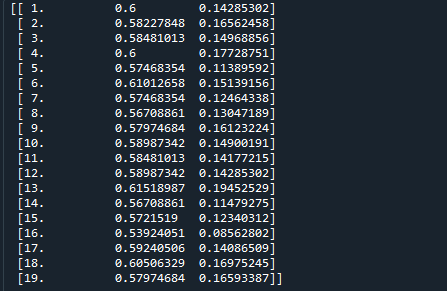
\includegraphics[width=10cm]{figures/1184071/chapter2/11-m.PNG}
		\caption{Hasil Soal 11.}
	\end{figure}
	\item Soal 12
	\hfill\break
	\lstinputlisting[firstline=145,lastline=153]{src/1184071/chapter2/1184071.py}
	Mengimport sebuah library dari matplotlib yaitu pylot sebagai plt fig dan ax menggunakan subplots untuk membuat gambar dan satu set subplot. axerrorbar akan membuat error bar kemudian grafik akan ditampilkan menggunakan show. Hasilnya adalah sebagai berikut :
	\begin{figure}
	\centering
		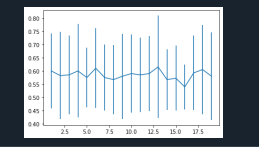
\includegraphics[width=10cm]{figures/1184071/chapter2/12-m.PNG}
		\caption{Hasil Soal 12.}
	\end{figure}
\end{enumerate}
\newpage\subsection{Penanganan Error}
\begin{enumerate}
	\item ScreenShoot Error
	\begin{figure}[h]
		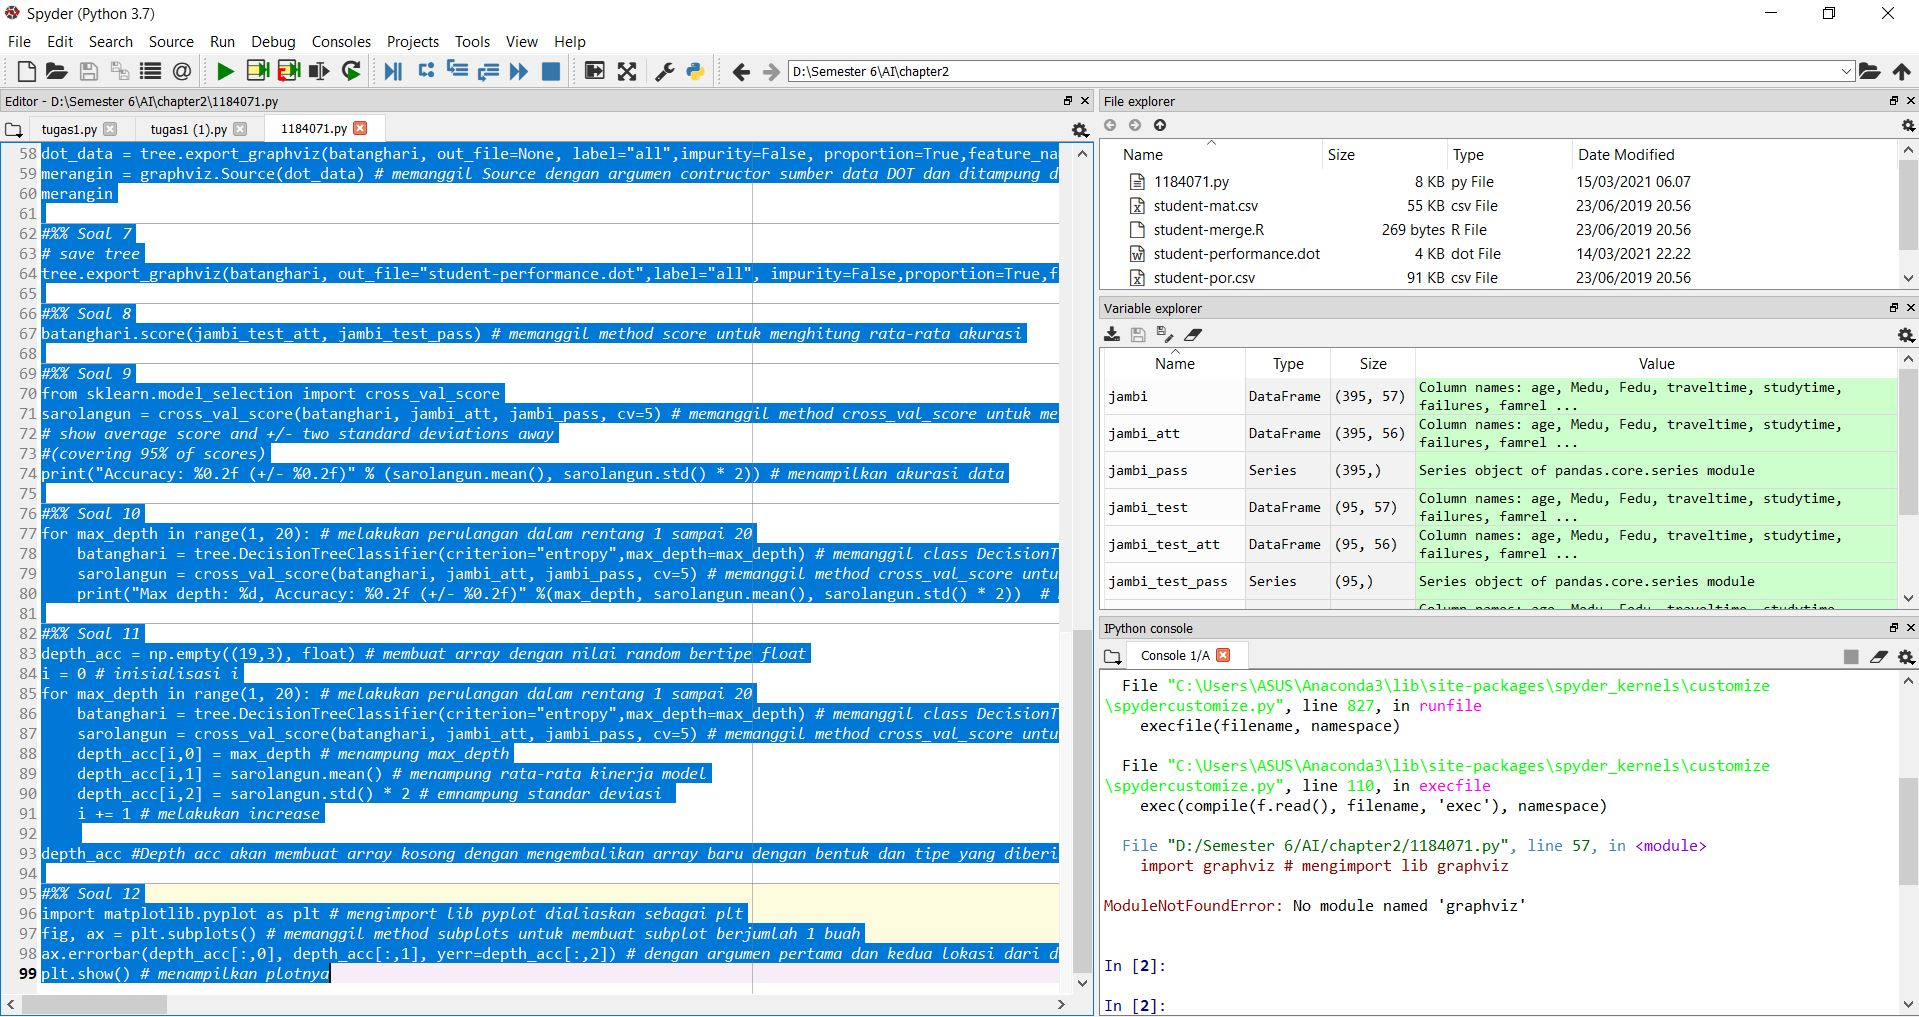
\includegraphics[width=8cm]{figures/1184071/chapter2/a.JPG}
		\centering
		\caption{ModuleNotFoundError}
	\end{figure}
	\item Tuliskan Kode Error dan Jenis Error
	\begin{itemize}
	\lstinputlisting[firstline=82, lastline=92]{src/1184071/chapter2/1184071.py}
		\item ModuleNotFoundError
	\end{itemize}
	\item Cara Penanganan Error
	\begin{itemize}
		\item ModuleNotFoundError
		\hfill\break
		Error terdapat pada kesalahan modul graphviz yang belum diinstall, solusinya ialah menginstall terlebih dahulu library tersebut di anaconda prompt.
	\end{itemize}
	\item Bukti Tidak Plagiarisme
	\begin{figure}[h]
		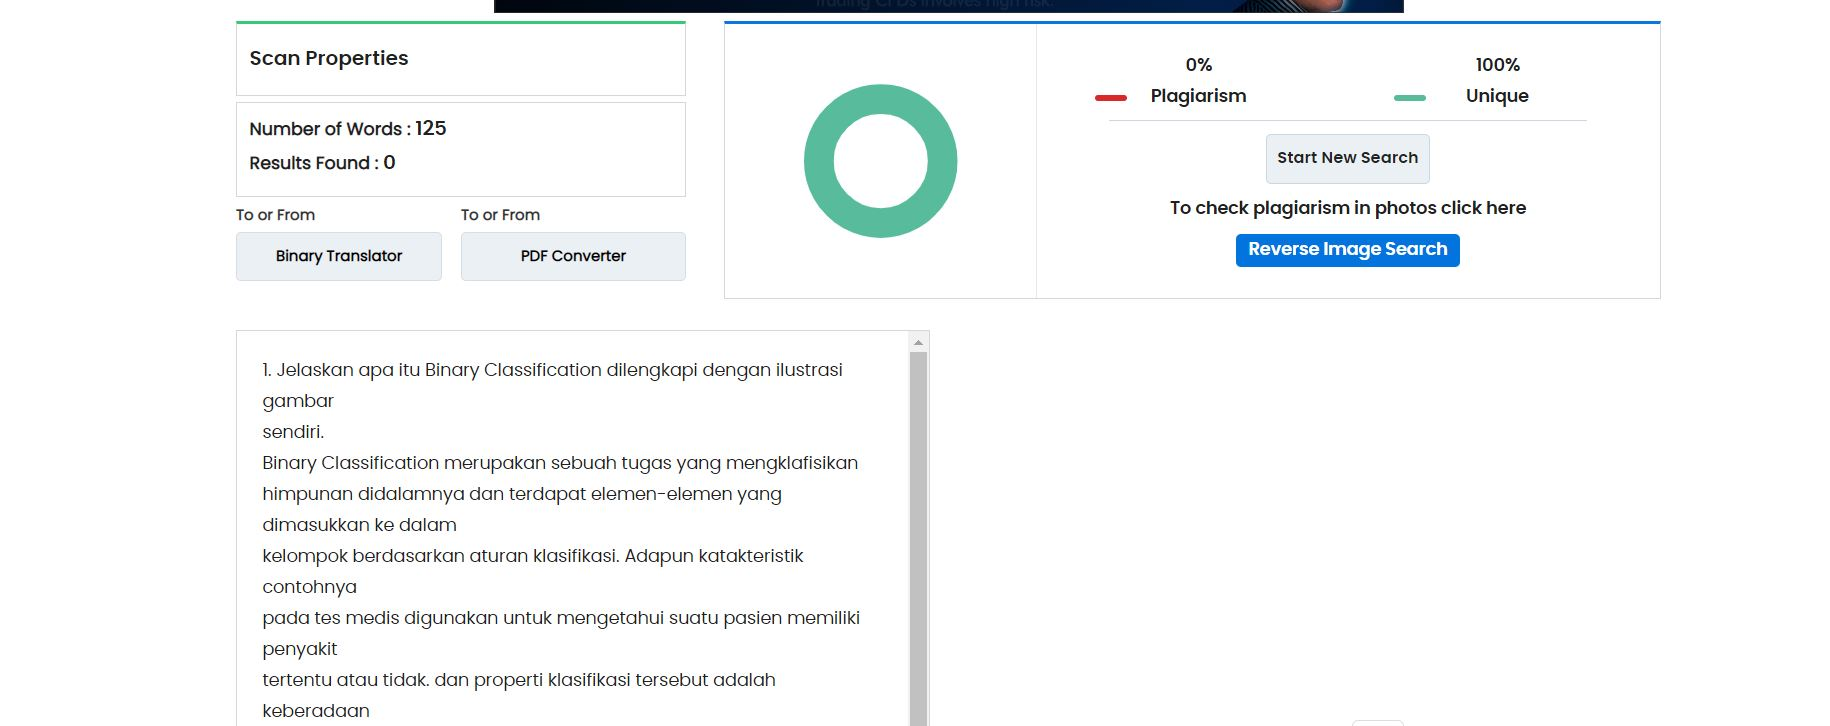
\includegraphics[width=12cm]{figures/1184071/chapter2/plagiat.JPG}
		\centering
		\caption{Bukti Tidak Melakukan Plagiat}
	\end{figure}
\end{enumerate}